% -*- TeX-engine: xetex; eval: (auto-fill-mode 0); eval: (visual-line-mode 1); -*-
% Compile with XeLaTeX

%%%%%%%%%%%%%%%%%%%%%%%
% To do before class
%%%%%%%%%%%%%%%%%%%%%%%

% Send the Logistics/Week0Annoucnement (the night before).
% Send an email reminding students to bring a charged computer (the night before).

%%%%%%%%%%%%%%%%%%%%%%%
% Option 1: Slides: (comment for handouts)   %
%%%%%%%%%%%%%%%%%%%%%%%

%\documentclass[slidestop,compress,mathserif,12pt,t,professionalfonts,xcolor=table]{beamer}
%
%% solution stuff
%\newcommand{\solnMult}[1]{
%\only<1>{#1}
%\only<2->{\red{\textbf{#1}}}
%}
%\newcommand{\soln}[1]{\textit{#1}}
%
%\newcommand{\solnMultOn}[3]{
%\only<#1>{#3}
%\only<{#2}->{\red{\textbf{#3}}}
%}

%%%%%%%%%%%%%%%%%%%%%%%%%%%%%%%
% Option 2: Handouts, without solutions (post before class)    %
%%%%%%%%%%%%%%%%%%%%%%%%%%%%%%%

 \documentclass[11pt,containsverbatim,handout,xcolor=xelatex,dvipsnames,table]{beamer}

 % handout layout
 \usepackage{pgfpages}
 \pgfpagesuselayout{4 on 1}[letterpaper,landscape,border shrink=5mm]

 % solution stuff
 \newcommand{\solnMult}[1]{#1}
 \newcommand{\soln}[1]{}
 \newcommand{\solnMultOn}[3]{#3}

 % % This breaks things for me for some reason.
 % tell pgfpages how to set page sizes in XeLaTeX
 \renewcommand\pgfsetupphysicalpagesizes{%
    \pdfpagewidth\pgfphysicalwidth\pdfpageheight\pgfphysicalheight%
 }

%%%%%%%%%%%%%%%%%%%%%%%%%%%%%%%%%%%%
% Option 3: Handouts, with solutions (may post after class if need be)    %
%%%%%%%%%%%%%%%%%%%%%%%%%%%%%%%%%%%%

% \documentclass[11pt,containsverbatim,handout,xcolor=xelatex,dvipsnames,table]{beamer}

% % handout layout
% \usepackage{pgfpages}
% \pgfpagesuselayout{4 on 1}[letterpaper,landscape,border shrink=5mm]

% % solution stuff
% \newcommand{\solnMult}[1]{\red{\textbf{#1}}}
% \newcommand{\soln}[1]{\textit{#1}}

% % % This breaks things for me for some reason.
% % % tell pgfpages how to set page sizes in XeLaTeX
% % \renewcommand\pgfsetupphysicalpagesizes{%
% %    \pdfpagewidth\pgfphysicalwidth\pdfpageheight\pgfphysicalheight%
% % }

%%%%%%%%%%%%%%%%%%%%%%%%%%%%%%%
% Option 4: Notes Only
%%%%%%%%%%%%%%%%%%%%%%%%%%%%%%%

% % See http://tex.stackexchange.com/questions/114219/add-notes-to-latex-beamer
% \documentclass[10pt,containsverbatim,xcolor=xelatex,dvipsnames,table,notes=only]{beamer}

% % handout layout
% % \usepackage{pgfpages}
% % \pgfpagesuselayout{1 on 1}[letterpaper, landscape, border shrink=5mm]

% % solution stuff
% \newcommand{\solnMult}[1]{#1}
% \newcommand{\soln}[1]{}

% % % Having a problem with this.
% % tell pgfpages how to set page sizes in XeLaTeX
% % \renewcommand\pgfsetupphysicalpagesizes{%
% %   \pdfpagewidth\pgfphysicalwidth\pdfpageheight\pgfphysicalheight%
% %}

%%%%%%%%%%
% Load style file, defaults  %
%%%%%%%%%%

%%%%%%%%%%%%%%%%
% Themes
%%%%%%%%%%%%%%%%

% See http://deic.uab.es/~iblanes/beamer_gallery/ for mor options

% Style theme
\usetheme{Pittsburgh}

% Color theme
\usecolortheme{seahorse}

% Helvetica Neue Light for most text
\usepackage{fontspec}
\setsansfont{Helvetica Neue Light}

%%%%%%%%%%%%%%%%
% Packages
%%%%%%%%%%%%%%%%

\usepackage{geometry}
\usepackage{graphicx}
\usepackage{amssymb}
\usepackage{epstopdf}
\usepackage{amsmath}  	% this permits text in eqnarray among other benefits
\usepackage{url}		% produces hyperlinks
\usepackage[english]{babel}
\usepackage{colortbl}	% allows for color usage in tables
\usepackage{multirow}	% allows for rows that span multiple rows in tables
\usepackage{color}		% this package has a variety of color options
\usepackage{pgf}
\usepackage{calc}
\usepackage{ulem}
\usepackage{multicol}
\usepackage{textcomp}
\usepackage{listings}
\usepackage{changepage}
\usepackage{tikz}
\usetikzlibrary{trees}		% for probability trees
\usepackage{fancyvrb}	% for colored code chunks
\usepackage{nameref}

%%%%%%%%%%%%%%%%
% Remove navigation symbols
%%%%%%%%%%%%%%%%

\beamertemplatenavigationsymbolsempty
\hypersetup{pdfpagemode=UseNone} % don't show bookmarks on initial view

%%%%%%%%%%%%%%%%
% User defined colors
%%%%%%%%%%%%%%%%

% Pantone 2015 Spring colors
% http://iwork3.us/2014/09/16/pantone-2015-spring-fashion-report/
% update each semester or year

\xdefinecolor{custom_blue}{rgb}{0, 0.70, 0.79} % scuba blue
\xdefinecolor{custom_darkBlue}{rgb}{0.11, 0.31, 0.54} % classic blue
\xdefinecolor{custom_orange}{rgb}{0.97, 0.57, 0.34} % tangerine
\xdefinecolor{custom_green}{rgb}{0.49, 0.81, 0.71} % lucite green
\xdefinecolor{custom_red}{rgb}{0.58, 0.32, 0.32} % marsala

\xdefinecolor{custom_lightGray}{rgb}{0.78, 0.80, 0.80} % glacier gray
\xdefinecolor{custom_darkGray}{rgb}{0.54, 0.52, 0.53} % titanium

%%%%%%%%%%%%%%%%
% Template colors
%%%%%%%%%%%%%%%%

\setbeamercolor*{palette primary}{fg=white,bg= custom_blue}
\setbeamercolor*{palette secondary}{fg=black,bg= custom_blue!80!black}
\setbeamercolor*{palette tertiary}{fg=white,bg= custom_blue!80!black!80}
\setbeamercolor*{palette quaternary}{fg=white,bg= custom_blue}

\setbeamercolor{structure}{fg= custom_blue}
\setbeamercolor{frametitle}{bg= custom_blue!90}
\setbeamertemplate{blocks}[shadow=false]
\setbeamersize{text margin left=2em,text margin right=2em}

%%%%%%%%%%%%%%%%
% Styling fonts, bullets, etc.
%%%%%%%%%%%%%%%%

% title slide
\setbeamerfont{title}{size=\large,series=\bfseries}
\setbeamerfont{subtitle}{size=\large,series=\mdseries}
%\setbeamerfont{institute}{size=\large,series=\mdseries}

% color of alerted text
\setbeamercolor{alerted text}{fg=custom_orange}

% styling of itemize bullets
\setbeamercolor{item}{fg=custom_blue}
\setbeamertemplate{itemize item}{{{\small$\blacktriangleright$}}}
\setbeamercolor{subitem}{fg=custom_blue}
\setbeamertemplate{itemize subitem}{{\textendash}}
\setbeamerfont{itemize/enumerate subbody}{size=\footnotesize}
\setbeamerfont{itemize/enumerate subitem}{size=\footnotesize}

% styling of enumerate bullets
\setbeamertemplate{enumerate item}{\insertenumlabel.}
\setbeamerfont{enumerate item}{family={\fontspec{Helvetica Neue}}}
\setbeamerfont{enumerate subitem}{family={\fontspec{Helvetica Neue}}}
\setbeamerfont{enumerate subsubitem}{family={\fontspec{Helvetica Neue}}}

% make frame titles small to make room in the slide
\setbeamerfont{frametitle}{size=\small} 

% set Helvetica Neue font for frame and section titles
\setbeamerfont{frametitle}{family={\fontspec{Helvetica Neue}}}
\setbeamerfont{sectiontitle}{family={\fontspec{Helvetica Neue}}}
\setbeamerfont{section in toc}{family={\fontspec{Helvetica Neue}}}
\setbeamerfont{subsection in toc}{family={\fontspec{Helvetica Neue}}, size=\small}
\setbeamerfont{footline}{family={\fontspec{Helvetica Neue}}}
\setbeamerfont{subsection in toc}{family={\fontspec{Helvetica Neue}}}
\setbeamerfont{block title}{family={\fontspec{Helvetica Neue}}}

%%%%%%%%%%%%%%%%
% New fonts accessed by fontspec package
%%%%%%%%%%%%%%%%

% Monaco font for code
\newfontfamily{\monaco}{Monaco}

%%%%%%%%%%%%%%%%
% Color text commands
%%%%%%%%%%%%%%%%

%orange
\newcommand{\orange}[1]{\textit{\textcolor{custom_orange}{#1}}}

% green
\newcommand{\green}[1]{\textit{\textcolor{custom_green}{#1}}}

% red
\newcommand{\red}[1]{\textit{\textcolor{custom_red}{#1}}}

% dark gray
\newcommand{\darkgray}[1]{\textit{\textcolor{custom_darkGray}{#1}}}

% light gray
\newcommand{\lightgray}[1]{\textit{\textcolor{custom_lightGray}{#1}}}

% pink
\newcommand{\pink}[1]{\textit{\textcolor{pink}{#1}}}


%%%%%%%%%%%%%%%%
% Custom commands
%%%%%%%%%%%%%%%%

% empty box for probability tree frame
\newcommand{\emptybox}[2]{
	\fbox{ \begin{minipage}{#1} \hfill\vspace{#2} \end{minipage} }
}

% cancel
\newcommand{\cancel}[1]{%
    \tikz[baseline=(tocancel.base)]{
        \node[inner sep=0pt,outer sep=0pt] (tocancel) {#1};
        \draw[red, line width=0.5mm] (tocancel.south west) -- (tocancel.north east);
    }%
}

% degree
\newcommand{\degree}{\ensuremath{^\circ}}

% cite
\newcommand{\ct}[1]{
\vfill
{\tiny #1}}

% Note
\newcommand{\Note}[1]{
\rule{2.5cm}{0.25pt} \\ \textit{\footnotesize{\textcolor{custom_red}{Note:} \textcolor{custom_darkGray}{#1}}}}

% Remember
\newcommand{\Remember}[1]{\textit{\scriptsize{\textcolor{custom_red}{Remember:} #1}}}

% links: webURL, webLink
\newcommand{\webURL}[1]{\urlstyle{same}{\textit{\textcolor{custom_blue}{\url{#1}}}}}
\newcommand{\webLink}[2]{\href{#1}{\textcolor{custom_blue}{{#2}}}}

% mail
\newcommand{\mail}[1]{\href{mailto:#1}{\textit{\textcolor{custom_blue}{#1}}}}

% highlighting: hl, hlGr, mathhl
\newcommand{\hl}[1]{\textit{\textcolor{custom_blue}{#1}}}
\newcommand{\hlGr}[1]{\textit{\textcolor{custom_green}{#1}}}
\newcommand{\mathhl}[1]{\textcolor{custom_blue}{\ensuremath{#1}}}

% example
\newcommand{\ex}[1]{\textcolor{blue}{{{\small (#1)}}}}

% two col: two columns
\newenvironment{twocol}[4]{
\begin{columns}[c]
\column{#1\textwidth}
#3
\column{#2\textwidth}
#4
\end{columns}
}

% slot (for probability calculations)
\newenvironment{slot}[2]{
\begin{array}{c} 
\underline{#1} \\ 
#2
\end{array}
}

% pr: left and right parentheses
\newcommand{\pr}[1]{
\left( #1 \right)
}

%%%%%%%%%%%%%%%%
% Custom blocks
%%%%%%%%%%%%%%%%

% activity: less commonly used
\newcommand{\activity}[2]{
\setbeamertemplate{itemize item}{{{\small\textcolor{custom_orange}{$\blacktriangleright$}}}}
\setbeamercolor{block title}{fg=white, bg=custom_orange}
\setbeamerfont{block title}{size=\small}
\setbeamercolor{block body}{fg=black, bg=custom_orange!20!white!80}
\setbeamerfont{block body}{size=\small}
\begin{block}{Activity: #1}
\setlength\abovedisplayskip{0pt}
#2
\end{block}
}

% app: application exercise
\newcommand{\app}[2]{
\setbeamercolor{block title}{fg=white,bg=custom_green}
\setbeamercolor{block body}{fg=black,bg=custom_green!20!white!80}
\begin{block}{{\small Application exercise: #1}}
#2
\end{block}
}

% disc: discussion question
\newcommand{\disc}[1]{
\vspace*{-2ex}
\setbeamercolor{block body}{bg=custom_blue!25!white!80, fg=custom_blue!55!black!95}
\begin{block}{\vspace*{-3ex}}
#1
\end{block}
\vspace*{-1ex}
}

% clicker: clicker question
\newcommand{\clicker}[1]{
\setbeamercolor{block title}{bg=custom_blue!80!white!50,fg=custom_blue!30!black!90}
\setbeamercolor{block body}{bg=custom_blue!20!white!80,fg=custom_blue!30!black!90}
\begin{block}{\vspace*{-0.2ex}{\footnotesize Clicker question}\vspace*{-0.2ex}}
#1
\end{block}
}

% formula
\newcommand{\formula}[2]{
\setbeamercolor{block title}{bg=custom_blue!40!white!60,fg=custom_blue!55!black!95}
\begin{block}{{\small#1}}
#2
\end{block}
}

% code
\newcommand{\Rcode}[1]{
{\monaco {\footnotesize \textcolor{custom_darkBlue}{#1}}}
}

% output
\newcommand{\Rout}[1]{
{\monaco {\footnotesize \textcolor{custom_darkGray}{#1}}}
}

%%%%%%%%%%%%%%%%
% Change margin
%%%%%%%%%%%%%%%%

\newenvironment{changemargin}[2]{%
\begin{list}{}{%
\setlength{\topsep}{0pt}%
\setlength{\leftmargin}{#1}%
\setlength{\rightmargin}{#2}%
\setlength{\listparindent}{\parindent}%
\setlength{\itemindent}{\parindent}%
\setlength{\parsep}{\parskip}%
}%
\item}{\end{list}}

%%%%%%%%%%%%%%%%
% Footnote
%%%%%%%%%%%%%%%%

\long\def\symbolfootnote[#1]#2{\begingroup%
\def\thefootnote{\fnsymbol{footnote}}\footnote[#1]{#2}\endgroup}

%%%%%%%%%%%%%%%%
% Graphics
%%%%%%%%%%%%%%%%

\DeclareGraphicsRule{.tif}{png}{.png}{`convert #1 `dirname #1`/`basename #1 .tif`.png}

%%%%%%%%%%%%%%%%
% Slide number
%%%%%%%%%%%%%%%%

\setbeamertemplate{footline}{%
    \raisebox{5pt}{\makebox[\paperwidth]{\hfill\makebox[20pt]{\color{gray}
          \scriptsize\insertframenumber}}}\hspace*{5pt}}

          
%%%%%%%%%%%%%%%%
% Remove page numbers
%%%%%%%%%%%%%%%%

\newcommand{\removepagenumbers}{% 
  \setbeamertemplate{footline}{}
}

%%%%%%%%%%%%%%%%
% TOC slides
%%%%%%%%%%%%%%%%

\setbeamertemplate{section in toc}{\inserttocsectionnumber.~\inserttocsection}
\setbeamertemplate{subsection in toc}{$\qquad$\inserttocsubsectionnumber.~\inserttocsubsection \\}

\AtBeginSection[] 
{ 
  \addtocounter{framenumber}{-1} 
  % 
  {\removepagenumbers 
  {\small
    \begin{frame}<beamer> 
    \frametitle{Outline} 
    \tableofcontents[currentsection] 
  \end{frame} 
  } 
  }
} 

\AtBeginSubsection[] 
{ 
  \addtocounter{framenumber}{-1} 
  % 
  {\removepagenumbers 
  {\small
    \begin{frame}<beamer> 
    \frametitle{Outline} 
    \tableofcontents[currentsection,currentsubsection] 
  \end{frame} 
  } 
  }
}
\input{../../definitions_default.tex}
% ALT ALT
%\input{../../definitions_custom.tex}

%%%%%%%%%%%
% Cover slide info    %
%%%%%%%%%%%

\title{Unit 7: Multiple linear regression}
\subtitle{3. Confidence and prediction intervals}
\author{Sta 101 - Spring 2015}
\date{April 13, 2015}
\institute{Duke University, Department of Statistical Science}

%%%%%%%%%%%
% Begin document   %
%%%%%%%%%%%

\begin{document}

%%%%%%%%%%%%%%%%%%%%%%%%%%%%%%%%%%%%

% Title Page

\begin{frame}[plain]

\titlepage
\vfill
{\scriptsize \webLink{\PersonalSite}{Dr. \LastName{}} \hfill Slides posted at  \webLink{\CourseSite}{\CourseSite}}
\addtocounter{framenumber}{-1} 

\end{frame}

%%%%%%%%%%%%%%%%%%%%%%%%%%%%%%%%%%%%

%\section{Housekeeping}
%
%%%%%%%%%%%%%%%%%%%%%%%%%%%%%%%%%%%%%
%
%\begin{frame}
%\frametitle{Announcements}
%
%\begin{itemize}
%
%\item 
%
%\end{itemize}
%
%\end{frame}
%
%%%%%%%%%%%%%%%%%%%%%%%%%%%%%%%%%%%%

\section{Uncertainty of predictions}

%%%%%%%%%%%%%%%%%%%%%%%%%%%%%%%%%%%%

\begin{frame}
\frametitle{Uncertainty of predictions}

\begin{itemize}

\item Regression models are useful for making predictions for new observations not include in the original dataset.

\pause

\item If the model is good, the predictions should be close to the true value of the response variable for this observation, however it may not be exact, i.e. $\hat{y}$ might be different than $y$.

\pause

\item With any prediction we can (and should) also report a measure of uncertainty of the prediction:
\begin{itemize}
\item Use a \hl{confidence interval} for the uncertainty around the expected value of predictions (average of a group of predictions) -- e.g. predict the average final exam score of a group of students who scored the same on the midterm.
\item Use a \hl{prediction interval} for the uncertainty around a single prediction -- e.g. predict the final exam score of one student with a given midterm score.
\end{itemize}

\end{itemize}

\end{frame}

%%%%%%%%%%%%%%%%%%%%%%%%%%%%%%%%%%%%

\subsection{Confidence intervals for average values}

%%%%%%%%%%%%%%%%%%%%%%%%%%%%%%%%%%%%

\begin{frame}
\frametitle{}

\formula{Confidence intervals for average values}{
A confidence interval for the average (expected) value of $y$, $E(y)$, for a given $x^\star$, is
\[ \hat{y} \pm t^\star_{n - 2} s \sqrt{ \frac{1}{n} + \frac{(x^\star - \bar{x})^2}{(n - 1)s_x^2} } \]
where $s$ is the standard deviation of the residuals, calculated as $\sqrt{\frac{\sum(y_i - \hat{y}_i)^2}{n-2}}$.
}

\end{frame}

%%%%%%%%%%%%%%%%%%%%%%%%%%%%%%%%%%%

\begin{frame}[fragile]
\frametitle{}

\disc{Calculate a 95\% confidence interval for the average IQ score of foster twins whose biological twins have IQ scores of 100 points. Note that the average IQ score of 27 biological twins in the sample is 95.3 points, with a standard deviation is 15.74 points.}
 
{\scriptsize
\begin{verbatim}
                 Estimate Std. Error t value Pr(>|t|)    
(Intercept)       9.20760    9.29990   0.990    0.332    
bioIQ             0.90144    0.09633   9.358  1.2e-09

Residual standard error: 7.729 on 25 degrees of freedom
\end{verbatim}
}

\twocol{0.4}{0.65}
{
\only<1|handout:0>{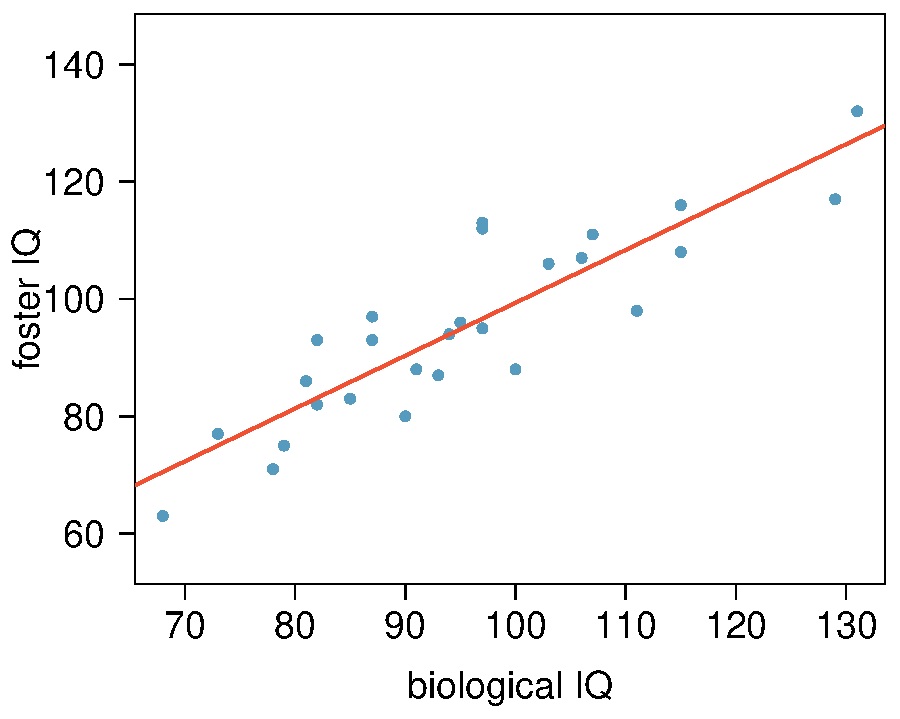
\includegraphics[width=\textwidth]{figures/twins/twins_IQ}}
\only<2-7|handout:0>{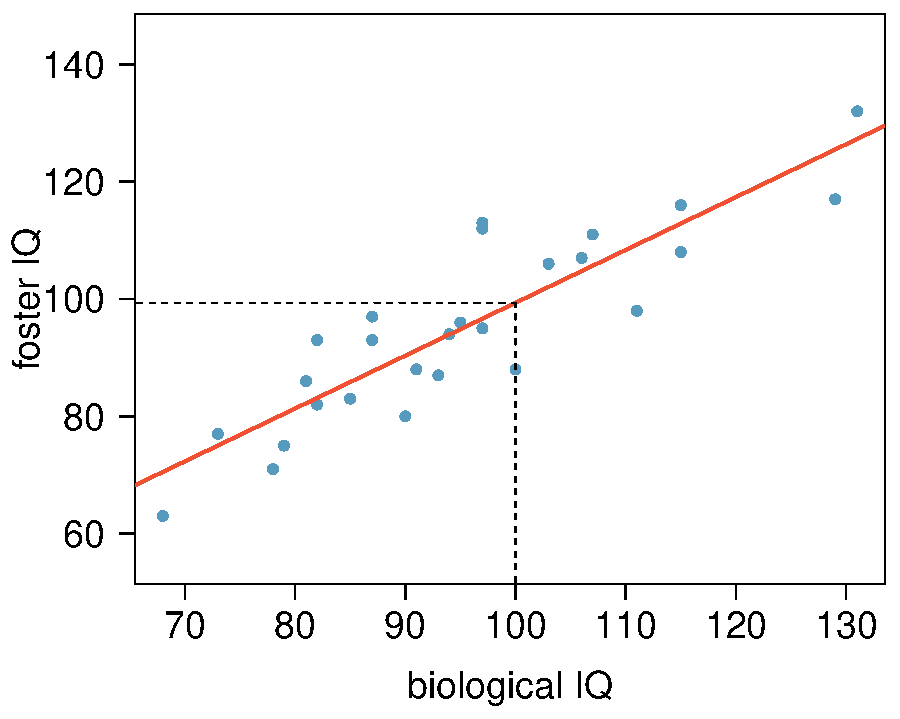
\includegraphics[width=\textwidth]{figures/twins/twins_IQ_100pred}}
\only<8>{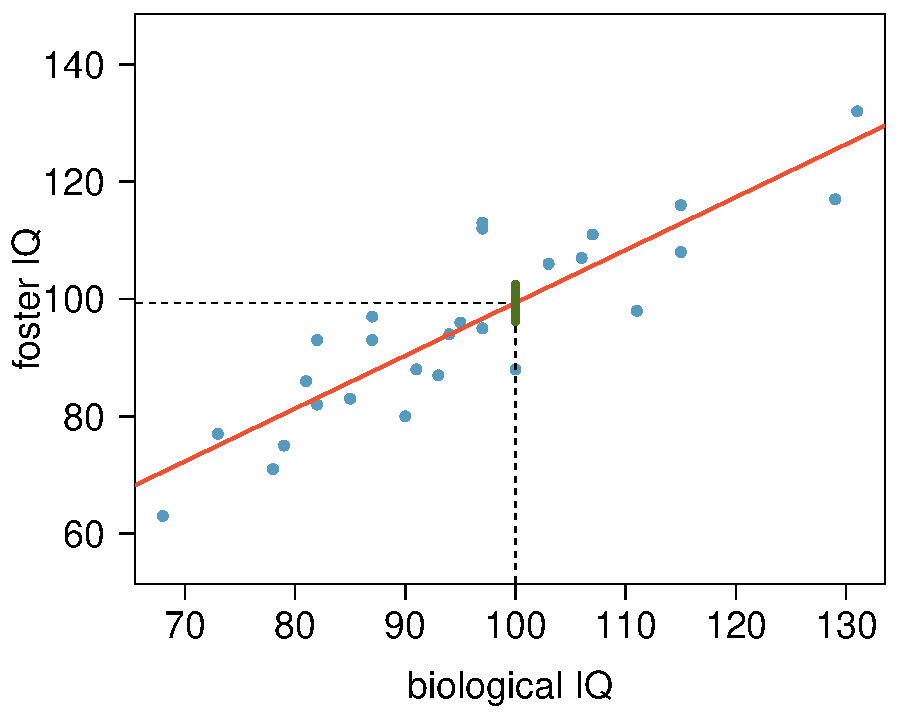
\includegraphics[width=\textwidth]{figures/twins/twins_IQ_100cint}}
}
{
\pause
{\small
\begin{eqnarray*}
\hat{y} &=& 9.2076 + 0.90144 \times 100 \approx 99.35 \\ \pause
df &=& n-2 \pause\qquad t^\star = 2.06 \\ \pause
ME &=& 2.06 \times 7.729 \times \sqrt{\frac{1}{27} + \frac{(100 - 95.3)^2}{26 \times 15.74^2}} \\ \pause
&\approx& 3.2 \\ \pause
CI &=& 99.35 \pm 3.2 \\ \pause
&=& (96.15, 102.55)
\end{eqnarray*}
}
}

\end{frame}

%%%%%%%%%%%%%%%%%%%%%%%%%%%%%%%%%%%

\begin{frame}[fragile]
\frametitle{Confidence interval for a prediction -- in R}

{\footnotesize
\begin{Verbatim}[frame=single, formatcom=\color{blue}]
# load data
install.packages("faraway") # dataset is in this package
library(faraway)
data(twins)

# fit model
m = lm(Foster ~ Biological, data = twins)

# create a new data frame for the new observation
newdata = data.frame(Biological = 100)

# calculate a prediction 
# and a confidence interval for the prediction
predict(m , newdata, interval = "confidence")
\end{Verbatim}
}

\pause

{\footnotesize
\begin{Verbatim}[frame=single, formatcom=\color{gray}]
     fit      lwr      upr
 99.3512 96.14866 102.5537
\end{Verbatim}
}

\end{frame}

%%%%%%%%%%%%%%%%%%%%%%%%%%%%%%%%%%%

\begin{frame}

\clicker{How would you expect the width of the 95\% confidence interval for the average IQ score of foster twins whose biological twins have IQ scores of 130 points ($x^\star = 130$) to compare to the previous confidence interval (where $x^\star = 100$)?}

\twocol{0.5}{0.5}
{
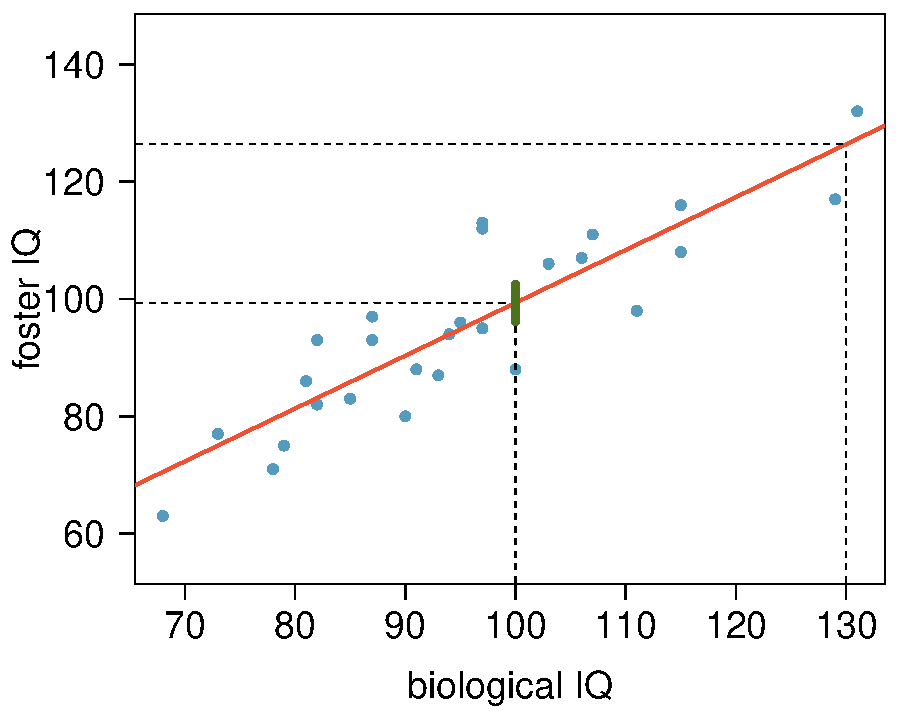
\includegraphics[width=\textwidth]{figures/twins/twins_IQ_100cint_130pred}
}
{
\begin{enumerate}[(a)]
\item \solnMult{wider}
\item narrower
\item same width
\item cannot tell
\end{enumerate}
}

\end{frame}


%%%%%%%%%%%%%%%%%%%%%%%%%%%%%%%%%%%

\begin{frame}[fragile]
\frametitle{}

\disc{How do the confidence intervals where $x^\star = 100$ and $x^\star = 130$ compare in terms of their widths?}
 
\twocol{0.2}{0.8}
{
\onslide<1->{\[ x^\star = 100 \]}
\onslide<2->{\[ x^\star = 130 \]}
}
{
\onslide<1->{\[ ME_{100} = 2.06 \times 7.729 \times \sqrt{\frac{1}{27} + \frac{(\red{100} - 95.3)^2}{26 \times 15.74^2}} = 3.2\]}
\onslide<3->{\[ ME_{130} = 2.06 \times 7.729 \times \sqrt{\frac{1}{27} + \frac{(\red{130} - 95.3)^2}{26 \times 15.74^2}} =}\onslide<4->{ 7.53 \]}
}

\onslide<5->{
\begin{center}
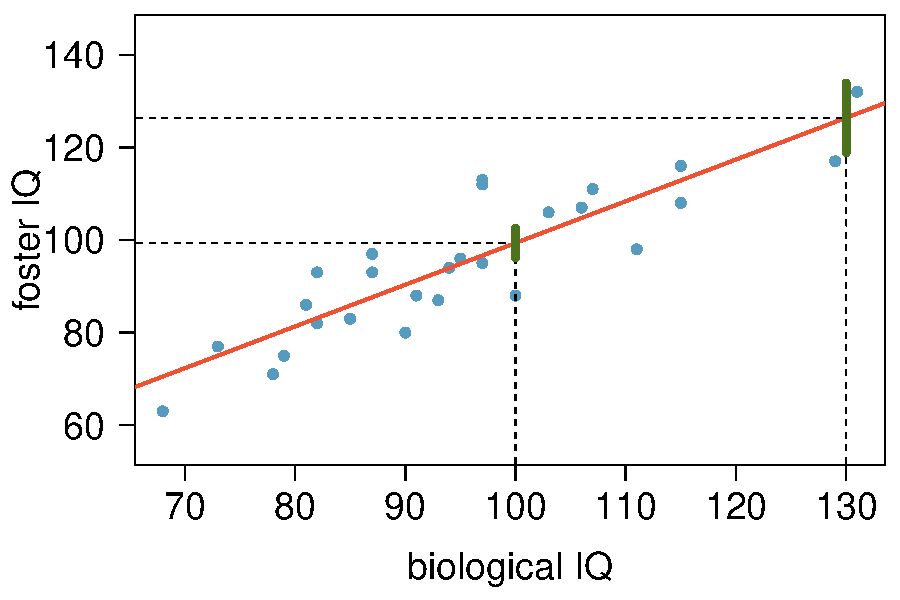
\includegraphics[width=0.5\textwidth]{figures/twins/twins_IQ_100cint_130cint}
\end{center}
}

\end{frame}


%%%%%%%%%%%%%%%%%%%%%%%%%%%%%%%%%%%

\begin{frame}
\frametitle{Recap}

\vspace{-0.25cm}

The width of the confidence interval for $E(y)$ increases as $x^\star$ moves away from the center.

\begin{itemize}

\item Conceptually: We are much more certain of our predictions at the center of the data than at the edges (and our level of certainty decreases even further when predicting outside the range of the data -- extrapolation).

\item Mathematically: As $(x^\star - \bar{x})^2$ term increases, the margin of error of the confidence interval increases as well.

\end{itemize}

\begin{center}
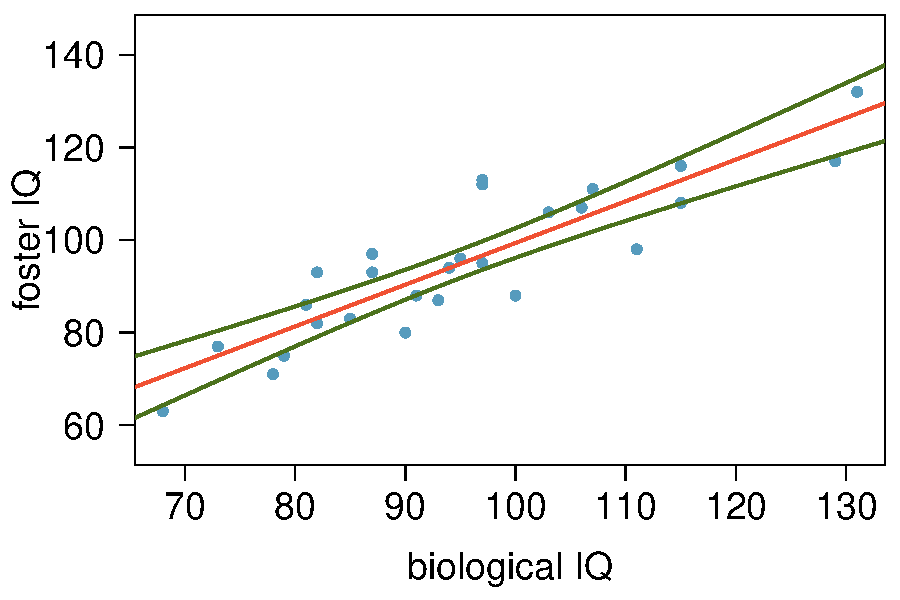
\includegraphics[width=0.5\textwidth]{figures/twins/twins_IQ_cint}
\end{center}

\end{frame}

%%%%%%%%%%%%%%%%%%%%%%%%%%%%%%%%%%%

\subsection{Prediction intervals for specific predicted values}

%%%%%%%%%%%%%%%%%%%%%%%%%%%%%%%%%%%%

\begin{frame}
\frametitle{}

\clicker{Earlier we learned how to calculate a confidence interval for average $y$, $E(y)$, for a given $x^\star$. \\

Suppose we're not interested in the average, but instead we want to predict a future value of $y$ for a given $x^\star$. \\

Would you expect there to be more uncertainty around an average or a specific predicted value?}

\begin{enumerate}[(a)]
\item more uncertainty around an average
\item \solnMult{more uncertainty around a specific predicted value}
\item equal uncertainty around both values
\item cannot tell
\end{enumerate}

\end{frame}

%%%%%%%%%%%%%%%%%%%%%%%%%%%%%%%%%%%%

\begin{frame}
\frametitle{}

\formula{Prediction intervals for specific predicted values}{
A \hl{prediction interval} for $y$ for a given $x^\star$ is
\[ \hat{y} \pm t^\star_{n - 2} s \sqrt{ 1 + \frac{1}{n} + \frac{(x^\star - \bar{x})^2}{(n - 1)s_x^2} } \]
where $s$ is the standard deviation of the residuals.
}

\pause

\begin{itemize}

\item The formula is very similar, except the variability is higher since there is an added 1 in the formula.

\pause

\item Prediction level: If we repeat the study of obtaining a regression data set many times, each time forming a XX\% prediction interval at $x^\star$, and wait to see what the future value of $y$ is at $x^\star$, then roughly XX\% of the prediction intervals will contain the corresponding actual value of $y$.

\end{itemize}

\end{frame}

%%%%%%%%%%%%%%%%%%%%%%%%%%%%%%%%%%%

\begin{frame}[fragile]
\frametitle{}

\vfill

\app{7.3 Prediction interval}{See course website for details}

\vfill

\soln{
\pause
We already found that $\hat{y} \approx 99.35$ and $t_{25}^\star = 2.06$. 
\begin{eqnarray*}
ME &=& 2.06 \times 7.729 \times \sqrt{1 + \frac{1}{27} + \frac{(100 - 95.3)^2}{26 \times 15.74^2}} \approx 16.24 \\ \pause
CI &=& 99.35 \pm 16.24 \\ \pause
&=& (83.11, 115.59)
\end{eqnarray*}
}

\end{frame}

%%%%%%%%%%%%%%%%%%%%%%%%%%%%%%%%%%%

\subsection{Recap - CI vs. PI}

%%%%%%%%%%%%%%%%%%%%%%%%%%%%%%%%%%%

\begin{frame}
\frametitle{CI for $E(y)$ vs. PI for $y$ (1)}

\begin{center}
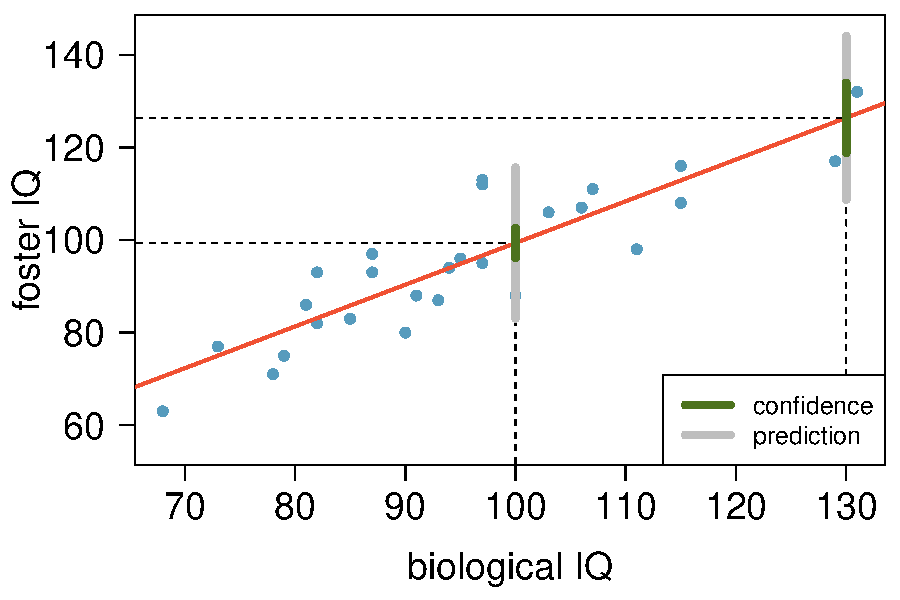
\includegraphics[width=\textwidth]{figures/twins/twins_IQ_100cintpint_130cintpint}
\end{center}

\end{frame}

%%%%%%%%%%%%%%%%%%%%%%%%%%%%%%%%%%%

\begin{frame}
\frametitle{CI for $E(y)$ vs. PI for $y$ (2)}

\begin{center}
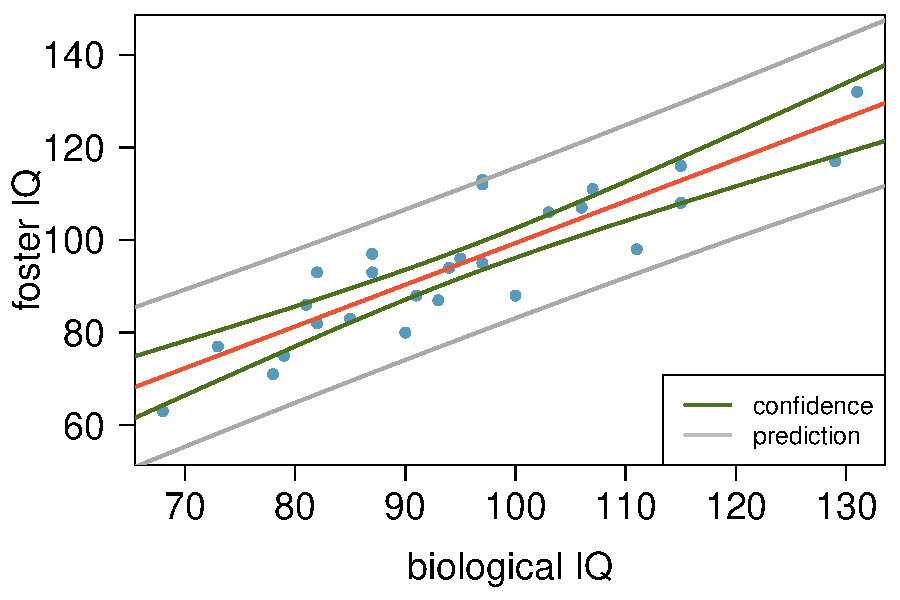
\includegraphics[width=\textwidth]{figures/twins/twins_IQ_cint_pint}
\end{center}

\end{frame}

%%%%%%%%%%%%%%%%%%%%%%%%%%%%%%%%%%%


\begin{frame}
\frametitle{CI for $E(y)$ vs. PI for $y$ - differences}

\begin{itemize}

\item A prediction interval is similar in spirit to a confidence interval, except that 
\pause
\begin{itemize}
\item the prediction interval is designed to cover a ``moving target", \\
the random future value of $y$, while
\pause
\item the confidence interval is designed to cover the ``fixed target", \\
the average (expected) value of $y$, $E(y)$,
\end{itemize}
for a given $x^\star$.

\pause

\item Although both are centered at $\hat{y}$, the prediction interval is wider than the confidence interval, for a given $x^\star$ and confidence level. This makes sense, since
\pause
\begin{itemize}
\item the prediction interval must take account of the tendency of $y$ to fluctuate from its mean value, while 
\pause
\item the confidence interval simply needs to account for the uncertainty in estimating the mean value.
\end{itemize}

\end{itemize}

\end{frame}

%%%%%%%%%%%%%%%%%%%%%%%%%%%%%%%%%%%

\begin{frame}
\frametitle{CI for $E(y)$ vs. PI for $y$ - similarities}

\begin{itemize}

\item For a given data set, the error in estimating $E(y)$ and $\hat{y}$ grows as $x^\star$ moves away from $\bar{x}$. Thus, the further $x^\star$ is from $\bar{x}$, the wider the confidence and prediction intervals will be.

\pause

\item If any of the conditions underlying the model are violated, then the confidence intervals and prediction intervals may be invalid as well. This is why it's so important to check the conditions by examining the residuals, etc.

\end{itemize}

\end{frame}

%%%%%%%%%%%%%%%%%%%%%%%%%%%%%%%%%%%

\subsection{Confidence and prediction intervals for MLR}

%%%%%%%%%%%%%%%%%%%%%%%%%%%%%%%%%%%

\begin{frame}
\frametitle{Confidence and prediction intervals for MLR}

\begin{itemize}

\item In the case of multiple linear regression (regression with many predictors), confidence and prediction intervals for a new prediction works exactly the same way.

\item However the formulas are much more complicated since we no longer have just one $x$, but instead many $x$s.

\item For confidence and prediction intervals for MLR we will focus on the concepts and leave the calculations up to R.

\end{itemize}

\end{frame}

%%%%%%%%%%%%%%%%%%%%%%%%%%%%%%%%%%%

\begin{frame}[fragile]
\frametitle{Prediction of evaluation my evaluation score}

\vspace{-0.2cm}

{\scriptsize
\begin{Verbatim}[frame=single, formatcom=\color{blue}]
load(url("http://www.openintro.org/stat/data/evals.RData"))

# fit a model
m = lm(score ~ rank + gender + language + 
    cls_perc_eval + cls_students, data = evals)

# create a data frame with the new observation (mine)
prof = data.frame(rank = "teaching", gender = "female", 
    language = "english", cls_perc_eval = 90, 
    cls_students = 120)
\end{Verbatim}
}

\pause

{\scriptsize
\begin{Verbatim}[frame=single, formatcom=\color{blue}]
predict(m , prof , interval = "prediction")
\end{Verbatim}
}

\pause

{\scriptsize
\begin{Verbatim}[frame=single, formatcom=\color{gray}]
       fit      lwr      upr
1 4.352334 3.315313 5.389355
\end{Verbatim}
}

\pause

{\scriptsize
\begin{Verbatim}[frame=single, formatcom=\color{blue}]
predict(m , prof , interval = "confidence")
\end{Verbatim}
}

\pause

{\scriptsize
\begin{Verbatim}[frame=single, formatcom=\color{gray}]
       fit      lwr      upr
1 4.352334 4.210043 4.494626
\end{Verbatim}
}

\end{frame}

%%%%%%%%%%%%%%%%%%%%%%%%%%%%%%%%%%%

\end{document}